
Alshahwan \etal ask the following: ``how long  should we wait, while continually observing no re-occurrence of a failure (in testing or production)
before we claim that the root cause(s) have been fixed?"~\cite{Facebook1}  Here, we assume the root cause(s) of a failure have been estimated by the work of WP1. The famous \textit{proving a negative problem} rears its head here: How we can prove a negative (no more failures) in the absence of direct evidence to the contrary.  
Alshahwan \etal state that identifying the correct \textit{fix detection protocol}~\cite{Facebook1} provides the solution, and experiment with their own protocol within the Sapienz Team
at Facebook. Their protocol uses heuristics and a finite state machine, but emphasize they ``do not claim it is the only possible protocol, nor that it is best among alternatives".  Accordingly, In this WP we propose the investigation of principled alternatives.

To begin our development, we propose to answer Alshawan's question above directly: We wait until we can claim a fix has occurred, i.e. when the error-causing behaviour of the method has diminished. 
Our answer is made precise as follows. 
We let the \textit{error causing behaviour} of a given method be a time series T = $t_1, t_2, \dots, t_n$, where each datapoint is an error-causing degree for a given failure group (as per WP2) over a given period. Let T1 = $t_1, t_2, \dots , t_k$ and T2 = $t_{k+1}, t_{k+2}, \dots , t_n$ be two adjacent time series splitting T.  Following the standard definition of changepoint detection, a \textit{changepoint} is detected for T1 and T2 if T1 and T2 are shown to be drawn from a different distribution according to a given hypothesis testing method~\citep{Aminikhanghahi, arXiv:1411.7955}.
We detect that some \textit{fix}/\textit{bug} has been introduced into T2 since T1, if i) a changepoint is detected for T1 and T2 and ii) the average error causing degree in T2 is smaller/larger than the average error causing degree in T1. Finally, we say the the error-causing behaviour of the method has \textit{diminished} when a fix is detected.

To illustrate the setup, consider~\autoref{f1}, which represents a time series of real-valued datapoints. Let T1 be the series before the vertical green line and T2 the series after. Already, our setup could be used to say some fix has been introduced into T2 since T1. It then remains to find the precise point where the fix was introduced. This is done by applying a changepoint detection method (CDM). In general, CDMs try to identify exact times (\textit{changepoints}) when the probability distribution of a stochastic process or time series can be confidently said to change. 
Ideally, we would apply a CDM which identifies the changepoint with the datapoint indicated by the green line in~\autoref{f1}.  
Research into CDMs is a large and well-developed area~\citep{Aminikhanghahi, arXiv:1411.7955}, and have been applied successfully to solve similar problems to FDP in continuous code deployment~\cite{arXiv:1411.7955}. Key differences between CDMs include where they locate changepoints, and how scalable the technique is. 





\begin{figure}[t!]
  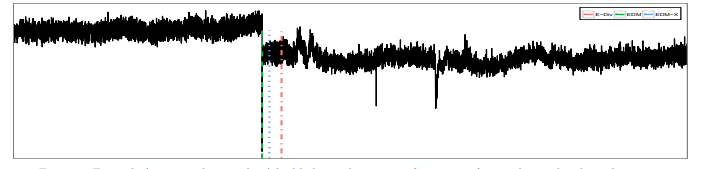
\includegraphics[width=\linewidth]{cp_z.png}
  \caption{Time Series with Change Point.}
  \label{f1}
  
\vspace*{-0.6cm}

\end{figure}


